\documentclass[12pt,letterpaper,noanswers]{exam}
\usepackage[usenames,dvipsnames,svgnames,table]{xcolor}
\usepackage[margin=0.9in]{geometry}
\renewcommand{\familydefault}{\sfdefault}
\usepackage{multicol}
\usepackage{wrapfig}
\pagestyle{head}
\definecolor{c03}{HTML}{FFDDDD}
\header{AM 22b Class 03}{}{Jan 29: contours + linear functions + $f(x,y,z)$}
\runningheadrule
\headrule
\usepackage{graphicx} % more modern
\usepackage{amsmath} 
\usepackage{amssymb} 
\usepackage{hyperref}
\usepackage{tcolorbox}

\usepackage[numbered,autolinebreaks,useliterate]{mcode}

\begin{document}
 \pdfpageheight 11in 
  \pdfpagewidth 8.5in


% I need to review the torus trajectories...

\begin{itemize}
\item There is a pre-class assignment (20 minutes of videos + a few WeBWorK exercises) due at 10am this Monday.  It will be available on Canvas at noon.
    \item Problem set 01 was released yesterday, and is due on Thurs Feb 4th at 6pm.  
    \item There is a skill check on Monday (for C02 and C03).  The C03 sample problem is in this handout (and C02 is in Wednesday's handout).
\end{itemize}

\hrule
\vspace{0.2cm}

\noindent\textbf{Big picture}

This week we will work with functions of multiple variables as well as with equations in three variables (chapter 12).  The goal is to become familiar with some common functions, equations, and surfaces, to identify correspondences between these, and to be able to interpret information about a function from graphical, analytical, and numerical representations of the information.

\vspace{0.2cm}
\hrule
\vspace{0.2cm}

\noindent\textbf{Skill Check C03 practice}
\begin{questions}
\item Find an expression for a level surface of the function \[f(x,y,z) = \ln{(x^2+3z^2)}.\]

Is the level surface a 

\begin{oneparcheckboxes}
\choice plane
\choice sphere or ellipsoid
\choice circular or elliptical paraboloid
\choice cylinder
\end{oneparcheckboxes}

\end{questions}


\vspace{0.2cm}

\hrule
\vspace{0.2cm}

\noindent\textbf{Skill Check C03 solution}

I set $\ln(x^2 + 3z^2) = c$.  Using $e$ to invert $\ln$, I have $x^2+3z^2 = e^c$.  Choose $c = 0$ as a convenient value to construct a single level surface, with $e^0 = 1$.  I have $x^2 + 3z^2 =1$ as an expression for one level surface of $f(x,y,z)$.

\begin{itemize}
    \item There are quadratic monomials in the level surface equation, so this isn't the equation for a plane.
    \item For a sphere or ellipsoid we would have $x^2$, $y^2$, $z^2$ all showing up, but we're missing $y^2$.
    \item Paraboloids are linear in one variable and quadratic in the other two, so the surface isn't a paraboloid.
    \item $y$ is missing from the expression, so this level surface will be a cylinder.  It is specifically an elliptical cylinder.
\end{itemize}

\vspace{0.2cm}
\hrule
\vspace{0.2cm}

\noindent\textbf{From C02}
\begin{itemize}
\itemsep0em
    \item Plotting a point
    \item Examples.
    \begin{itemize}
    \itemsep0em
        \item function.  $f: (x,y) \mapsto x^2+y^2$.
        \item equation.  $z = x^2 + y^2$.
        \item graph of $f$ (and solution set of equation).  $\{(x,y,z): z = x^2+y^2\}$
    \end{itemize}
    \item Specifying a curve in $3$-space.
    \begin{itemize}
    \itemsep0em
        \item $\left\{\begin{array}{c}x= 0 \\ z = 0\end{array}\right.$ or  $\left\{\begin{array}{c}x + z = 0 \\ z = 0\end{array}\right.$ (equivalent systems).  Specifies points $\{(0,y,0)\}$ (for any $y\in \mathbb{R}$)
        \item $\left\{\begin{array}{c}x^2+y^2 + (z-4)^2= 9 \\ z = 2\end{array}\right.$ or  $\left\{\begin{array}{c}x^2 + y^2 = 5 \\ z = 2\end{array}\right.$ (equivalent systems).
    \end{itemize}
\end{itemize}

\vspace{0.2cm}
\hrule
\vspace{0.2cm}

\noindent\textbf{Contour plots} \S 12.3
\begin{tcolorbox}
%\textbf{For your reference (section 12.3):} \\
For a function $f(\underline{x})$ the set of points $\underline{x}$ such that $f(\underline{x}) = c$ is called the $c$-\textbf{level set} of the function.  Note: the $c$-level set is a set in the domain of $f$.

The $c$-level set for a function of two variables is a set in $2$-space, and is often called a \textbf{level curve} or a \textbf{contour line}.  

If we choose a regular interval, $k$ (called the \textbf{contour interval}), and draw the set of level curves $..., c-k, c, c+k, c+2k, ...$ in the $2$-space, we call the resulting diagram a \textbf{contour diagram}.  Two contour diagrams are shown below.

The $c$-level set for a function of three variables is a set in $3$-space, and is often called a \textbf{level surface}.  



% \emph{production functions}

\end{tcolorbox}




Note: if a point $(x,y)$ is in the $c$-level set, it is not in the (c+1)-level set.  Why not? \\

\noindent\textbf{Examples.}

Mount Greylock, on the left, is the highest point in Massachusetts.

\begin{center}
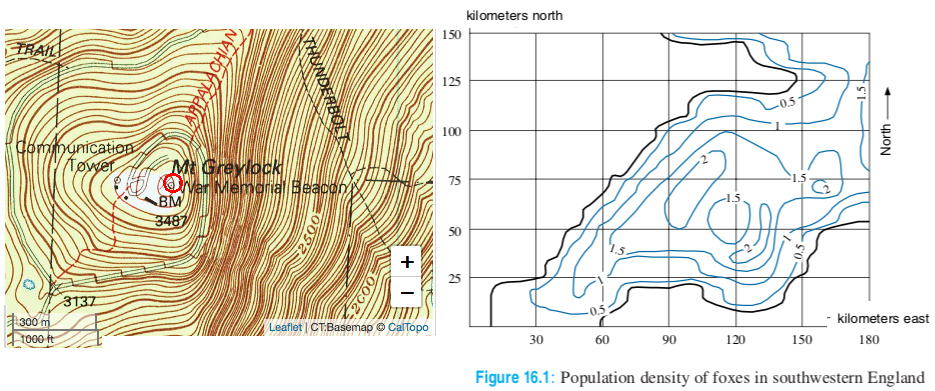
\includegraphics[width=0.9\linewidth]{img/C03contours.png}
\end{center}


\vspace{0.2cm}
\hrule
\vspace{0.2cm}

\noindent\textbf{Graph vs level set}

In the table below, $x,y,z$ are variables, $f$ is a scalar function, and $c$ is a constant.

\begin{tabular}{|c|c|c|c|c|}
\hline
function & graph & space of graph & level sets & space of level sets\\
 &  & (domain,output) &  & (domain)\\
\hline
  $f:x\mapsto f(x)$   & $\{(x,f(x))\}$ & curve in $2$-space & $f(x) = c$ & points  in $1$-space\\
   $f:(x,y)\mapsto f(x,y)$  & $\{(x,y,f(x,y))\}$ & surface in $3$-space & $f(x,y) = c$ & curves  in $2$-space\\
   $f:(x,y,z)\mapsto f(x,y,z)$  & $\{(x,y,z,f(x,y,z))\}$ & solid in $4$-space & $f(x,y,z)=c$ & surfaces in $3$-space \\
   \hline
\end{tabular}

\vspace{0.2cm}
\hrule
\vspace{0.2cm}
\eject

\noindent\textbf{Teams}
\begin{multicols}{3}
1.  student names
\end{multicols}

Share a fruit or vegetable that you like with the members of your team.

\vspace{0.2cm}
\hrule
\vspace{0.2cm}

\noindent\textbf{Examples}

 Identify the shape of the contour lines for each of the following functions: 
\begin{itemize}
    \item $f(x,y) = y - x^2$.  Contours are of the form $y - x^2 = c$, so parabolas in $xy$-space.
    \item $f(x,y) = x^2$
    \vspace{0.7cm}
    
    \item $f(x,y) = x^2+2y^2$
       \vspace{0.7cm}
       
        \item $f(x,y) = e^{-(x^2+2y^2)}$
       \vspace{0.7cm}
       
    \item $f(x,y) = y^2 - x^2$
       \vspace{0.7cm}
       
\end{itemize}
 


% \textbf{asymptotic}
% \textbf{radial symmetry}
% \textbf{cylinder}
% \textbf{production function}


\vspace{0.2cm}
\hrule
\vspace{0.2cm}


\vspace{0.2cm}
\hrule
\vspace{0.2cm}
\begin{tcolorbox}
To draw a \textbf{contour diagram} for a function $f(x,y)$, choose evenly spaced values of $c$ (the spacing is the \textbf{contour interval}).  Draw the contours corresponding to each value of $c$ in the domain of the function (in $2$-space for a function of two variables).
\end{tcolorbox}

Construct a contour diagram for $f(x,y) = 2x^2 + y^2.$

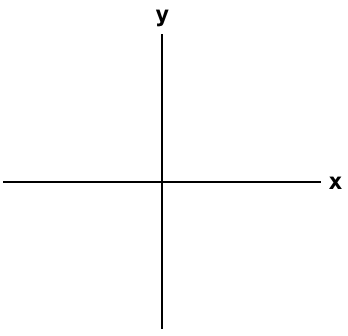
\includegraphics[scale=0.6]{img/C02axes-2.png}

\vspace{0.2cm}
\hrule
\vspace{0.2cm}


\eject

\noindent\textbf{Matlab code example 1}
\begin{lstlisting}
%% contour plot method 1
f1 = @(x,y) y.*x.^2; % use .* and .^, not just * and ^, in case x, y is a vector input.
syms x y
fcontour(f1(x,y),[0, 2, 0, 2])
xlabel('x'); ylabel('y');
axis equal
print('-opengl','~/Desktop/C03p1a.png','-dpng','-r300')
\end{lstlisting}

\noindent\textbf{Matlab code example 2}
\begin{lstlisting}
%% contour plot method 2
f1 = @(x,y) y.*x.^2;
[x1,y1] = meshgrid(0:0.1:2,0:0.1:2);
contour(x1, y1, f1(x1,y1))
xlabel('x'); ylabel('y');
axis equal
print('-opengl','~/Desktop/C03p1b.png','-dpng','-r300')
\end{lstlisting}

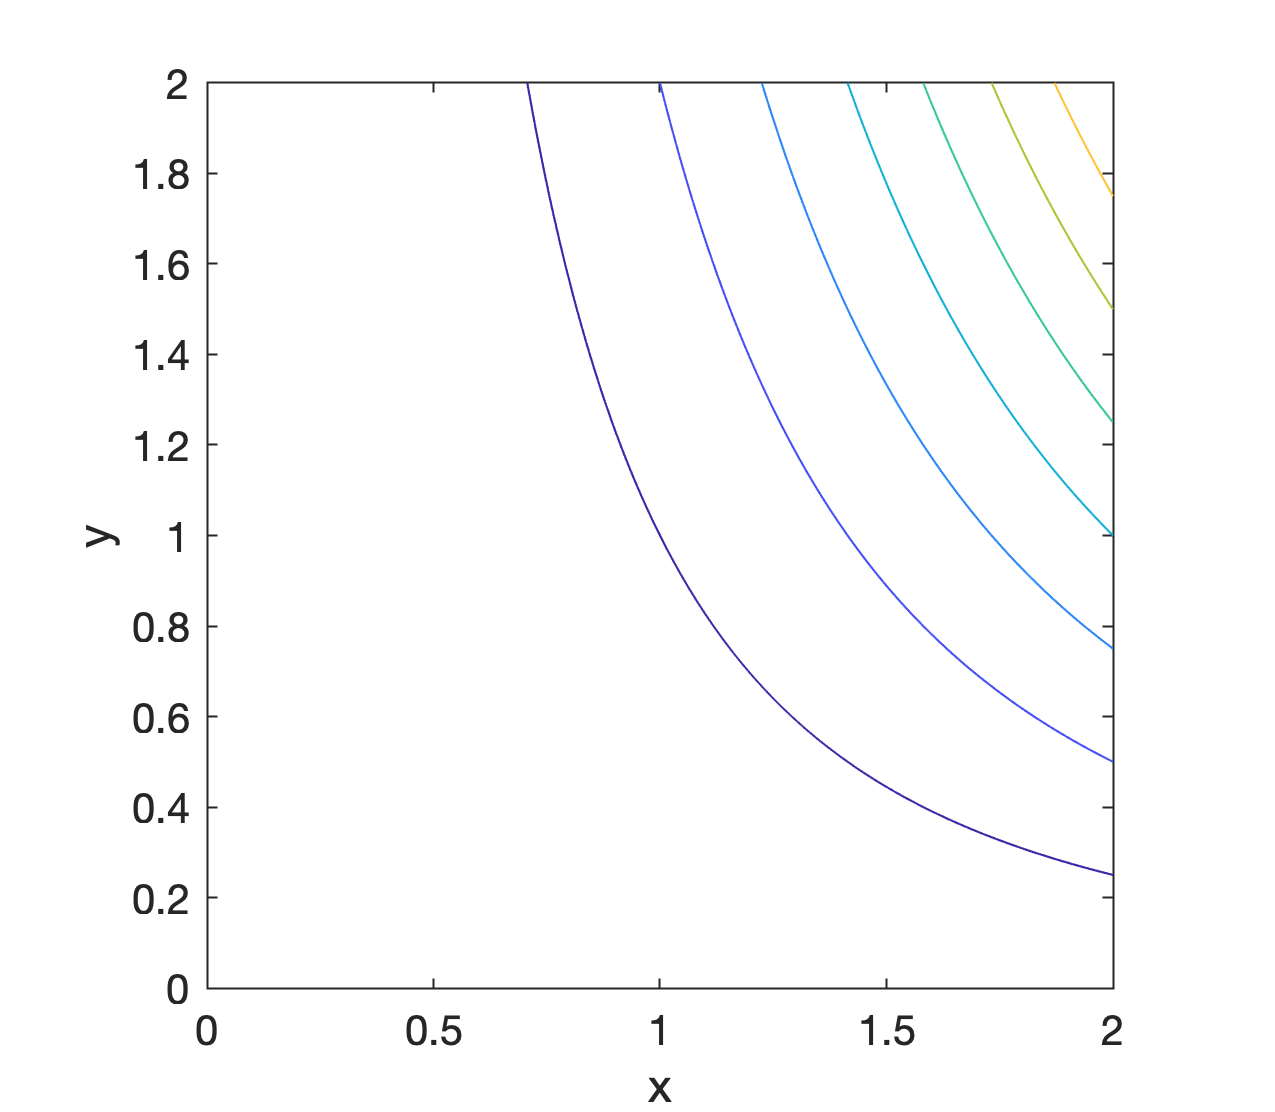
\includegraphics[width=3in]{img/C03p1a.png}

\vspace{0.2cm}
\hrule
\vspace{0.2cm}

\eject
\noindent\textbf{Linear functions} \S 12.4

Here are some ways of constructing an equation for a line in $2$-space:
\begin{itemize}
    \item $y = mx + b$ (slope-intercept form)
    \item $(y-y_0) = m(x-x_0)$ (point-slope form)
    \item $x/a+y/b = 1$ (intercept form)
    \item From Calculus Blue: \url{https://www.youtube.com/watch?v=M4xOUmgBbmc}
\end{itemize}

\noindent\textbf{Example}:
Sketch the graph of $x/2 + y/3 = 1$ in $xy$-space and in $xyz$-space.

\hfill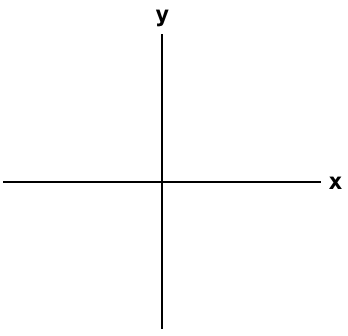
\includegraphics[height=3in]{img/C02axes-2.png}\hfill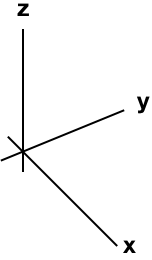
\includegraphics[height=3in]{img/C02axes.png}\hfill

Here are some ways of constructing an equation for a plane in $3$-space:
\begin{itemize}
    \item $z = mx + ny + b$ ('slope'-intercept form)
    \item $n_x(x-x_0) + n_y(y-y_0) +n_z(z-z_0) = 0$ (point-'slope' form).  
    \item $x/a+y/b + z/c= 1$ (intercept form)
    \item From Calculus Blue: \url{https://www.youtube.com/watch?v=xAEYKHW6D48}
\end{itemize}

Lines and planes are linear objects.

\begin{tcolorbox}
Definitions vary a little, but for the purposes of this course we'll use the term \textbf{monomial} to refer to a polynomial with only one term.  You can think of a polynomial with multiple terms as the sum of monomials.

The \textbf{degree} of a monomial is the sum of the exponents of the variables making up the monomial: $x^ay^bz^2$ has degree $a+b+2$.

The \textbf{degree} of a polynomial is the maximum degree of its terms.

A \textbf{linear equation} is an equation that can be obtained by setting a linear polynomial to zero.

A \textbf{linear function} is a polynomial function that is the sum of monomials of degree $0$ or $1$.


The \textbf{contour diagram} for a linear function of two variables, $f(x,y) = mx + ny + b$, consists of evenly spaced, parallel, lines. 

\end{tcolorbox}

\eject
\noindent\textbf{Example}:
\begin{itemize}
    \item Is $f(x,y) = 2x + 3y + 7$ a linear equation?
    \vspace{0.6cm}
    
    \item Is $2x+3y+7 = 0$ a linear equation?
    \vspace{0.6cm}

\item Rewrite $3x+2y +2 = 0$ in intercept form.  Use intercept form to sketch the graph of this equation in $2$-space.

\hfill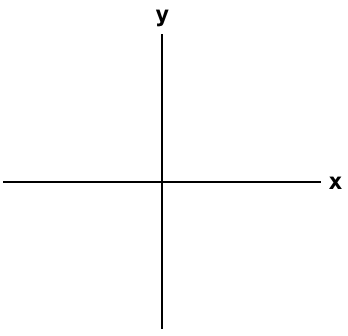
\includegraphics[height=3in]{img/C02axes-2.png}\hfill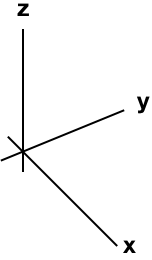
\includegraphics[height=3in]{img/C02axes.png}\hfill

\item Rewrite $3x+2y-5z +2 = 0$ in intercept form.  Use intercept form to sketch the graph of this equation in $3$-space.
\vspace{1cm}

\end{itemize}

\vspace{3in}

\vspace{0.2cm}
\hrule
\vspace{0.2cm}

\noindent\textbf{Surfaces} \S 12.5

\begin{tcolorbox}
A \textbf{quadratic equation} is an equation that can be obtained by setting a polynomial of degree $2$ to zero.

A \textbf{quadratic function} is a polynomial function that is the sum of monomials of degree $0$, $1$, or $2$.

A \textbf{homogeneous polynomial} is a polynomial whose terms each have the same degree.

A \textbf{quadratic form} is a homogeneous polynomial of degree $2$.
\end{tcolorbox}



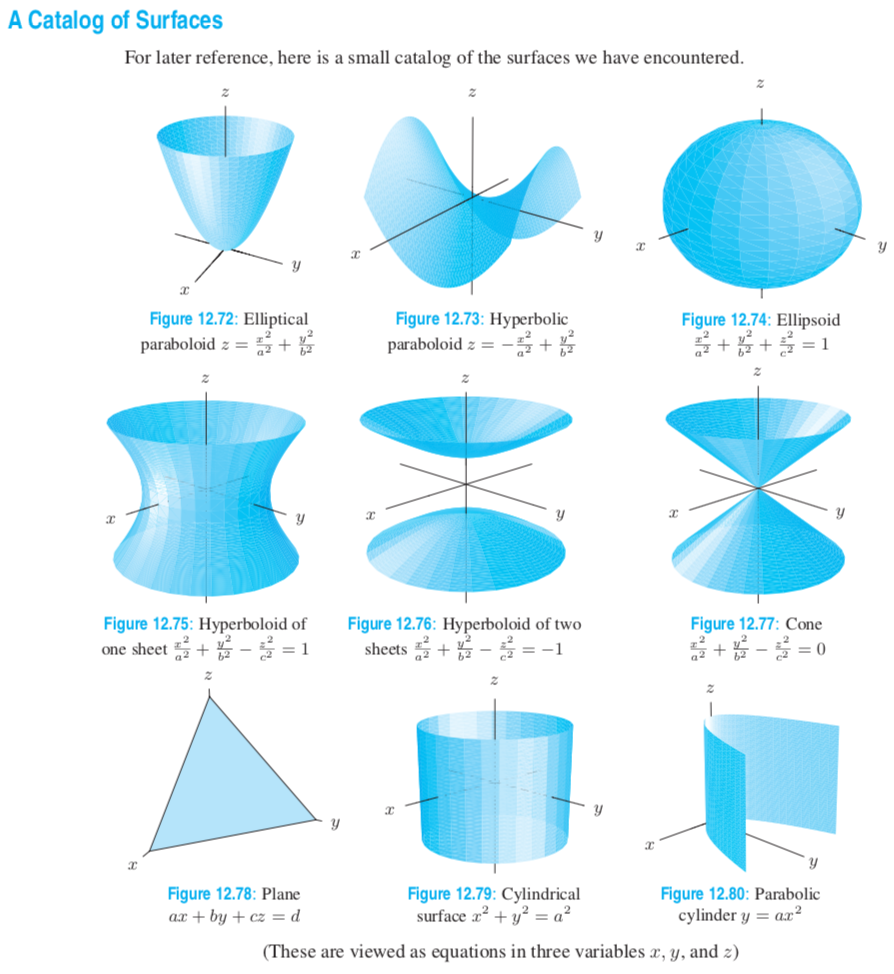
\includegraphics[width=\textwidth]{img/C05surfaces.png}


\noindent\textbf{Example.}  Let $f(x,y,z) = x^2 + y^2 + z$.  The $c$-level set is the set of points that satisfy $x^2+y^2 +z = c$.  We have $z = c - x^2 - y^2.$ This is a circular paraboloid centered about the $z$-axis and opening downward, with a maximum value of $c$.
\vspace{0.3cm}



\vspace{0.2cm}
\hrule
\vspace{0.2cm}





\end{document}